\section{Ejercicio 4: Metaheurística}

  % \begin{figure}[ht]
  %   \begin{center}
  %     \includegraphics[width=0.5\columnwidth]{imagenes/pacman.png}
  %     \caption{Perdidos y con poca fuerza}
  %   \end{center}
  % \end{figure}

    % 1. Describir detalladamente el problema a resolver dando ejemplos del mismo y sus soluciones.
    \subsection{Descripción del problema y solución propuesta}
        En este punto, se pidió realizar un algoritmo basado en una metaheurística que resuelva el problema en cuestión. El mismo al tratarse de una metaheurística puede no dar la solución óptima, y puede no devolver una solución aunque la misma exista.

    % 2. Explicar de forma clara, sencilla, estructurada y concisa, las ideas desarrolladas para la resolución del problema. Utilizar pseudocódigo y lenguaje coloquial (no código fuente). Justificar por qué el procedimiento resuelve efectivamente el problema.
        Se decidió utilizar como metaheurística para resolver esta variante del TSP, GRASP. De esta forma se explora el espacio de soluciones, partiendo de diferentes intancias y tratando de mejorarlas mediante búsqueda local. La idea de GRASP es que cada búsqueda va a converger en caso de ser posible a un mínimo local. Como se comienza de distintas instancias se van a explorar varios mínimos locales distintos, con lo cual la solución se puede obtener tomando la mejor de estas buenas soluciones. Como la eficacia de GRASP depende de empezar de soluciones lo suficientemente diferentes utiliza una heurística greedy a la que le suma aleatoridad, en la cual en vez de seleccionar siempre al mejor candidato para una solución, selecciona uno al azar de un grupo de candidatos (el RCL), cuyo tamaño o criterio de selección es configurable. La otra parte configurable de GRASP es la determinación de cuánto se va a buscar, es decir, cuanto tiempo se va a invertir en generar soluciones greedy aleatoria y tratar de mejorarlas. Para este caso particular de este problema, la implementación de GRASP elegida consiste en lo siguiente: se obtiene una solución (en caso de ser posible) mediante una heurística greedy. La misma es similar a la desarrollada en el ejercicio 2. La diferencia es que se le agrega aleatoridad, ya que no se toma a la estación más cercana sino que se eligen k estaciones más cercanas (siendo k un parámetro configurable) y se elige una al azar de esas estaciones. La misma estación elegida tiene que ser factible de ser visitada. En caso contrario, el algoritmo devuelve que no encontró solución. Si se toma como parámetro k = 1, este algoritmo greedy es exactamente igual al desarrollado en el ejercicio 2 ya que en todas las iteraciones va a elegir al más cercano. Si se toma como k la cantidad de estaciones total, el algoritmo se transforma en uno completamente aleatorio ya que en cada iteración se toma cualquiera estación. Luego de obtenerse una solución a la misma se le aplica la búsqueda local desarrollada en el ejercicio 3 para tratar de mejorarla. Este procedimiento se repite varias veces hasta que se cumple la condición de parada (parámetro configurable). Se usaron dos condiciones de parada distintas: una es determinar una cantidad de repeticiones que se desea realizar el procedimiento (condición sobre la cantidad de repeticiones del ciclo) y la otra es una cantidad de repeticiones en la cual no se mejoró una solución (condición sobre la cantidad de repeticiones sin mejorar). En ambos casos siempre el algoritmo termina ya que en el primer caso se fija la cantidad de repeticiones (por lo tanto el ciclo corre un número finito de veces) y en el otro aunque se elija un número muy grande, siempre a partir de un momento la solución no se va a poder mejorar (cuando se encuentra la óptima), por lo que en el peor caso si la óptima es encontrada rápidamente por el algoritmo, se va ejecutar una vez encontrada, la cantidad de iteraciones fijada, ya que no se va a poder encontrar ninguna mejor. En cada paso, se va guardando la solución mejor que se encuentra. Es decir, se mantiene una solución, que se actualiza en caso de que se encuentre una mejor en cada iteración de este procedimiento. Al finalizar se retorna la mejor solución encontrada.

        El algoritmo propuesto es el siguiente:

         \begin{codesnippet}
            \begin{verbatim}
solverEj4(vector<Estacion> estaciones, vector<vector<double> > distancias, n, m,
          k, grasp, <int, bool> criterio, bool vecindarioBusqLocal) {
  solucion s1
  solucion s2
  solucion best
  i = 0
  bool mejor
  double nuevaSol

  mientras (i < criterio.first)
    s1 = greedyRandomized(estaciones, distancias, n, m, k, grasp)
    s2 = solucionEj3(s1, estaciones, distancias, k, vecindarioBusqLocal)

    mejor = false
    nuevaSol = get<0>(s2)
    si i == 0  ó (nuevaSol > -1 && nuevaSol < get<0>(best)) 
      best = s2
      si (i > 0) 
        mejor = true
      
    
    si (!criterio.second)
      i++
    si no
      si (!mejor)
        i++
  fin mientras
  devolver best
            \end{verbatim}
            \end{codesnippet}


        El algoritmo consiste en un ciclo, el cual se ejecuta mientras no se haya llegado a la condición de terminación. La condición de terminación está dada por una tupla (denominada criterio) que contiene en su primer coordenada un entero, que es el que se usa en la condición del ciclo para saber si hay que cortar o no. La segunda coordenada es un booleano y sirve para identificar cual de los dos criterios que definimos se está utilizando. El booleano si es verdadero indica que se usa el criterio de parar cuando no se pudo mejorar en k veces la solución siendo k el entero de la primera coordenada. Si es falso, significa que se usa el criterio de correr directamente k veces el ciclo, siendo k también el entero de la primer coordenada.
        En el cuerpo del ciclo lo que se realiza es obtener una solución llamando a la función \textit{greedyRandomized}, la cual realiza lo mismo que la implementada en el ejercicio 2, salvo que en vez de seleccionar a la estación más cercana a la que se puede ir en cada paso, selecciona una al azar de n estaciones cercanas, siendo n el entero \textit{grasp} que se le pasa a la función. Luego de eso se aplica búsqueda local, llamando a la función \textit{solucionEj3}, la cual es exactamente la misma que la desarrollada en el ejercicio 3. Si nos encontramos en la primera iteración del ciclo o la solución obtenida es mejor que la anterior que teniamos, entonces se actualiza la nueva mejor solución obtenida con la encontrada en esta iteración.
        Finalmente se pregunta si se está usando el criterio de ejecutar k veces fijo (con lo cual la variable \textit{criterio.second} sería falsa) y en caso de ser así se suma uno al contador del ciclo. Sino, se trata del otro criterio y sólo se actualiza el contador si no se encontró una mejor solución en la iteración (hecho representado por el valor de la variable booleana \textit{mejor}), sumándole 1.
        Una vez terminado el ciclo se devuelve la mejor solución obtenida.

  \subsection{Experimentación}

    Para poder comparar cada configuración posible y obtener de ahí la configuración óptima. Se fijó una instancia la cual tenía 8 pokeparadas y 8 gimnasios, además de fijar el tamaño de la mochila para asegurar que siempre haya solución. Esto se hizo para poder comparar en una misma instancia todas las posibles configuraciones. La instancia mencionada es:

\begin{codesnippet}
  \begin{verbatim}
         8 8 24
         1 1 1
         2 2 2
         3 3 3
         4 4 1
         5 5 2
         6 6 3
         7 7 1
         8 8 2
         9 9
         10 10
         11 11
         12 12
         13 13
         14 14
         15 15
         16 16
  \end{verbatim}
\end{codesnippet}

Luego se realizaron dos experimentos. En el primero, se iteró sobre la cantidad de vértices que entrarán en la RCL, lista en la cual se randomiza, para obtener alguna nueva estacion. Mientras que en el segundo, se iteró sobre el límite de cada criterio de parada. Para ambos al igual que en el \textbf{Ejercicio 3}, se buscó comparar por un lado, qué configuración devolvía valores óptimos, además de qué configuración corría en menor tiempo. En cada gráfico se usaron las siguientes referencias, P = Criterio de paradas, i = Iteraciones del criterio, V = vecindario de búsqueda local, RCL = K vértices que accederan a la RCL.

\subsubsection{Experimento 1: RCL}

En el siguiente experimento, se crearon 4 instancias, las mismas mantenían los gimnasios y pokeparadas anteriormente mencionados. Mientras que por cada instancia se modificó el vecindario utilizado en la Búsqueda Local y el criterio de parada (la cantidad de iteraciones se fijó en 100).

De esta manera las siguientes 4 instancias son 

\begin{table}[H]
\centering
\begin{tabular}{ |c|c|c| } 
 \hline
 Instancias&Busqueda Local&Criterio de parada\\ 
 \hline
 Instancia 0 & Vecindario A & Iterar K veces\\
 \hline
 Instancia 1 & Vecindario A & Iterar hasta K peores\\
 \hline
 Instancia 2 & Vecindario B & Iterar K veces \\
 \hline
 Instancia 3 & Vecindario B & Iterar hasta K peores\\
 \hline
\end{tabular}
\caption{Instancias experimento 1}
\end{table}


Luego por cada instancia, se iteró el K de RCL, de 1 a 16. Por cada K, se corrió 100 veces el mismo algoritmo, y se sacó un promedio del tiempo y de la distancia. De esta manera para cada K, se calculó cuánto tiempo tardó el algoritmo además de la calidad de solucion. Luego, los resultados fueron, 


  \begin{figure}[H]
      \begin{center}
        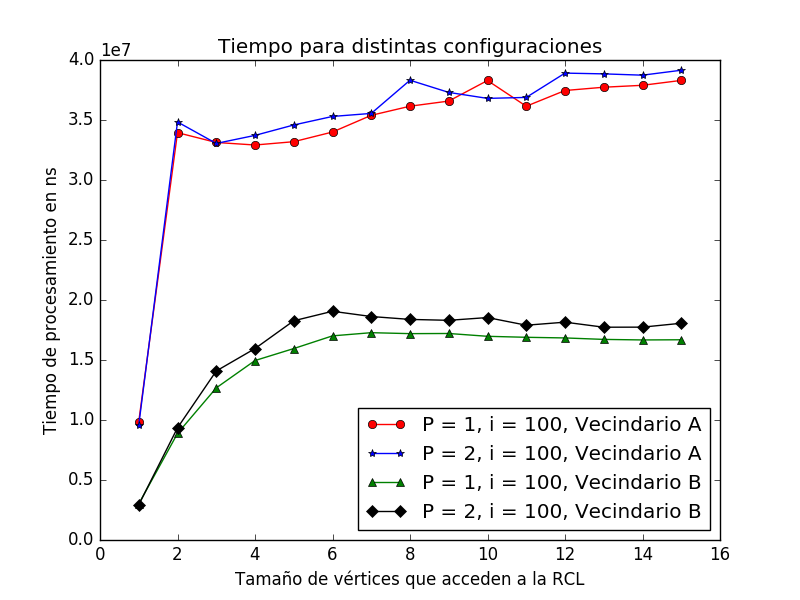
\includegraphics[width=0.7\columnwidth]{imagenes/Exp1TIempoEJ4.png}
      \end{center}
  \end{figure}


  Luego, a partir de esta experimentación, pudimos observar que a medida que crecía la lista RCL, el algoritmo obtenía mayor posibilidad de random. Esto generó una mayor tardanza a medida que crecía el K. Por otro lado, pudimos observar que otro aspecto que influye en el tiempo de corrida, fue vecindario utilizado. Nuevamente como fue mencionado en \textbf{Ejercicio 3}, debido a que intercambiar gimnasios en los recorridos, genera menos soluciones (pues caer en un recorrido válido intercambiando gimnasios con distintas pociones es muy poco probable). Luego, intercambiar pokeparadas, dado que no puede suceder que intercambiar en una solución pokeparadas, caiga en un recorrido válido, entonces cualquier intercambio puede llegar a ser un posible mínimo local. Luego en primer lugar, observamos que a menor K, tiene menos tiempo de corrida. Por otro lado, el vecindario B corre en menor tiempo que el A.

\begin{figure}[H]
    \begin{center}
      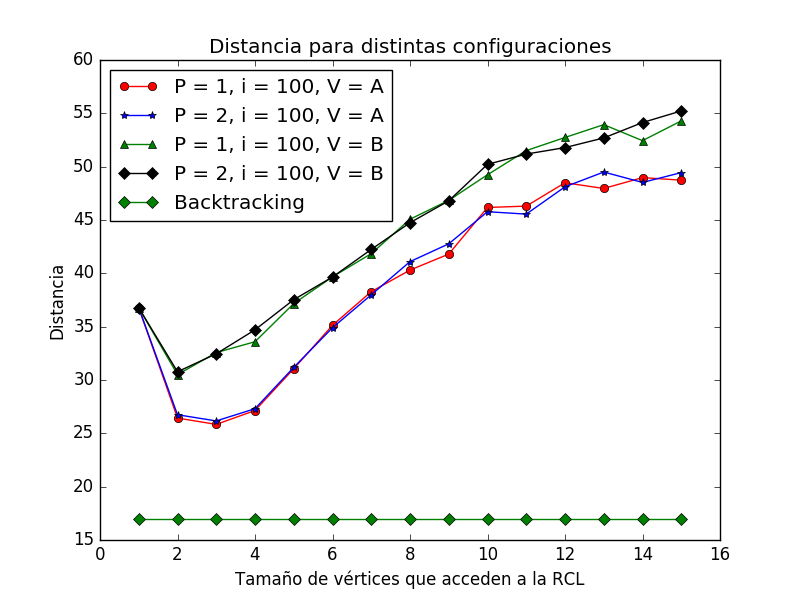
\includegraphics[width=0.7\columnwidth]{imagenes/Exp1DistanciaEj4.png}
    \end{center}
\end{figure}

Para este nuevo experimento comparamos la calidad de la solución. Por un lado observamos que con un menor RCL, las soluciones son óptimas. Por otro lado, observamos que los criterios de parada no generan una diferencia destacable en cuanto a performance en los algoritmos. Luego, el vecindario A, si bien corre en más tiempo que el B, genera mejores soluciones. Mejor es para un tamaño de RCL pequeño.


\subsubsection{Experimento 2: Iterar el límite de los criterios de parada}

Para este segundo experimento, se usaron las mismas instancias, con la diferencia que se fijó el RCL en 5, además de iterar de 1 a 100 el límite de ambos criterios de parada.


\begin{figure}[H]
    \begin{center}
      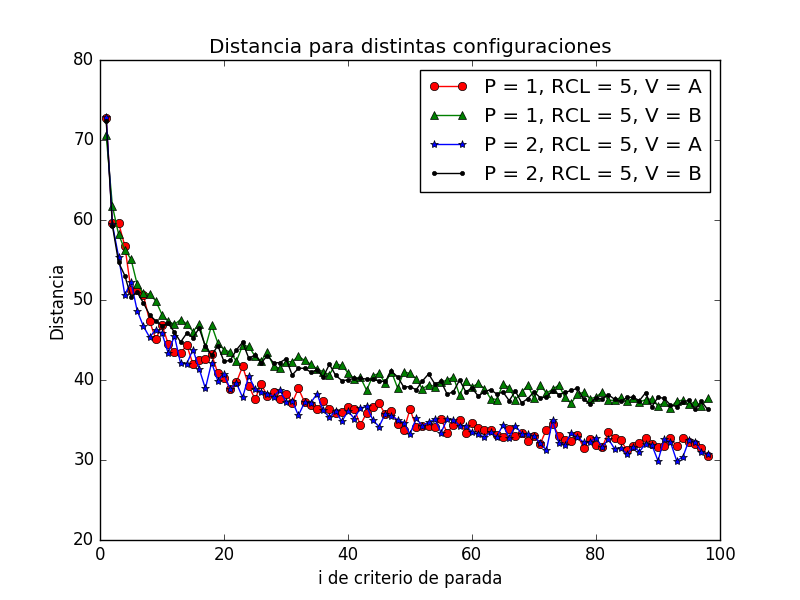
\includegraphics[width=0.7\columnwidth]{imagenes/Exp2DistanciaEj4.png}
    \end{center}
\end{figure}

\begin{figure}[H]
    \begin{center}
      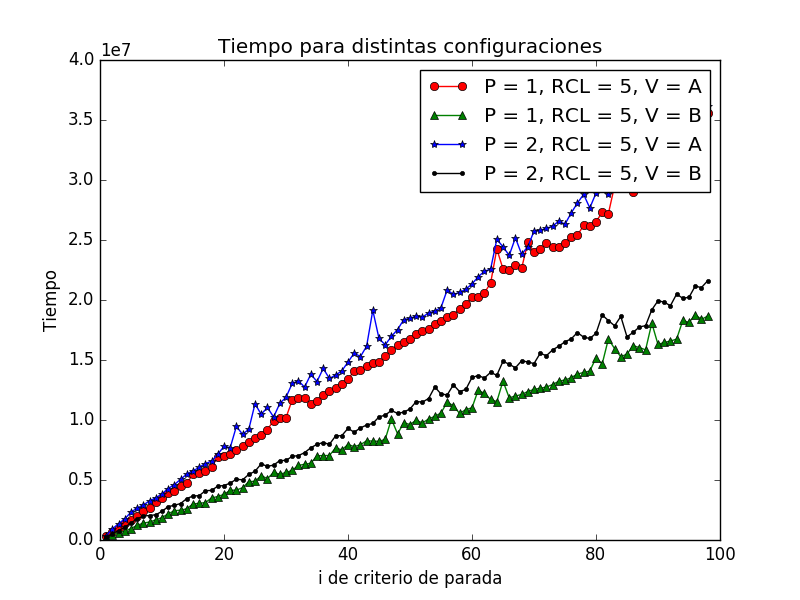
\includegraphics[width=0.7\columnwidth]{imagenes/Exp2TiempoEj4.png}
    \end{center}
\end{figure}


En primer lugar, en el primer gráfico como fue esperado, a mayor cantidad de iteraciones de criterio de parada, son mayores las soluciones recorridas dentro del campo de solución. Es por esto que es más probable que se encuentren mejores soluciones.

\par Por otro lado, en términos de tiempo, como fue esperado si la cantidad de iteraciones de la metaheurística crece, el tiempo de corrida crece linealmente.

\par Finalmente comparamos ambos criterios de parada cada uno con una vecindad distinta


\begin{figure}[H]
\minipage{0.5\textwidth}
  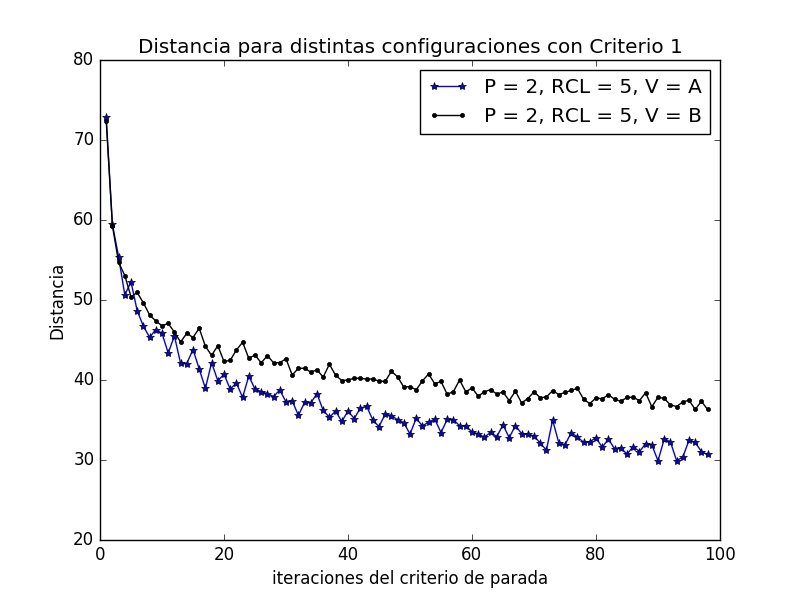
\includegraphics[width=\linewidth]{imagenes/Exp2Ej2DistanciaCrit1.png}
  \caption{Criterio 1}
\endminipage\hfill
\minipage{0.5\textwidth}%
  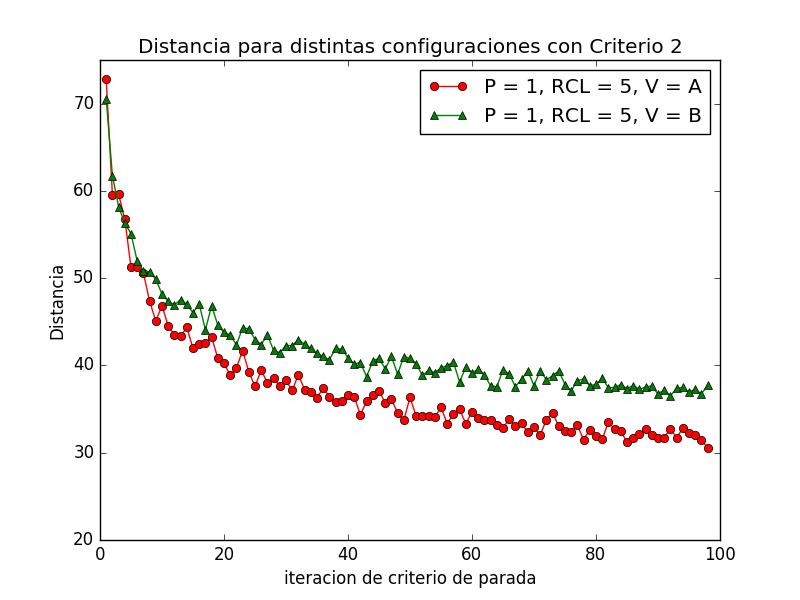
\includegraphics[width=\linewidth]{imagenes/Exp2Ej2DistanciaCrit2.png}
  \caption{Criterio 2}
\endminipage
\end{figure}



Se observa que nuevamente, la selección del vecindario es determinante a la hora de una mejor solución.
